%%% Local Variables:
%%% mode: latex
%%% TeX-master: t
%%% End:

%%%%%%%%%%%%%%%%%%%% Preamble %%%%%%%%%%%%%%%%%%%%

\documentclass[11pt, paper=a4]{article}
\usepackage[utf8]{inputenc}
\usepackage{amssymb,amsfonts,amsmath,latexsym,amsthm, mathtools} %mathtext,
\usepackage{booktabs}
\usepackage{multirow}
\usepackage{graphicx}
\usepackage{listings}
\usepackage{chngpage}
\usepackage{cprotect}
\usepackage[font=footnotesize, labelsep=period]{caption}
\usepackage{cite}
\usepackage[scale=0.8]{geometry}
\usepackage[pdftex,unicode,colorlinks, citecolor=blue,
filecolor=black, linkcolor=blue, urlcolor=blue]{hyperref}
\usepackage[figure,table]{hypcap}
\usepackage{setspace}

\graphicspath{{images/}}
\onehalfspacing{}

%%%%%%%%%%%%%%%%%%%% Document %%%%%%%%%%%%%%%%%%%%

\begin{document}

%%%%%%%%%%%%%%%%%%%% Title page %%%%%%%%%%%%%%%%%%%%

\title{{Report 2}\\{\bf Regression and Classification}}

\author{Markus Færevaag {\tt s123692} \& Jonathan Becktor {\tt s123094}}

\date{\today}

\maketitle

\begin{abstract}
  In this assignment we will explore Linear regression (LR), linear
  regression with forward selection (FLR), decision trees (DT), k
  nearest neighbors (KNN), naive bayes (NB), artificial neural networks
  (ANN), and multinomial regression (MNMR) methods.


  %% For regression
  %% problem, we found that the ANN model performs best, and the FLR and
  %% the average age (AVE) models are indistinguishable from each
  %% other. For classification problem, we found the ANN and MNMR to be the
  %% best performing models, and showed them to perform better than the
  %% largest class (LCl) classifier and the linear regression models (LR)
  %% using the paired t-test.
  %% Objective: The objective of this second report is to apply the
  %% methods you have learned in the second section of the course on
  %% ”Supervised learning: Classification and regression” in order to
  %% solve both a relevant classification and regression problem for your
  %% data.
\end{abstract}

%%%%%%%%%%%%%%%%%%%% Introduction %%%%%%%%%%%%%%%%%%%%
\section{Regression}
\label{sec:regression}
\subsection{Group issue}
Initially we were three people in our group. But due to our last group
member not finishing her part, and not letting us know that she would not
finish her part of the assignment, some of the answers will be
missing/lackluster. This is the second time she does not do
anything and now she no longer replies to our message. We have
therefore decided to remove her from our group.


\subsection{Problem description}
We have selected the regession problem detect spam emails from regular
emails given 57 features.  The features used are wordfrequencies of 54
different words/signs, the amount of capital letters, the longest
sequence of capital letters and the average and the average sequence
of capital letters.

\subsection{Linear Regression with forward selection}
As our dataset has 57 features it is infeasable to compare them all.
Therefore for the for this section only the 12 first features are used.
The 12 features.

Firstly we check if there are any obvious relationships between the
different features and if its spam or not. It is hard to tell if there
is a distinct relationship between the features. If any of them have a
linear relationship they can be reduced to a single feature. (see figure1)

\begin{figure}[h]
  \begin{minipage}{0.3\textwidth}
    a)\\
    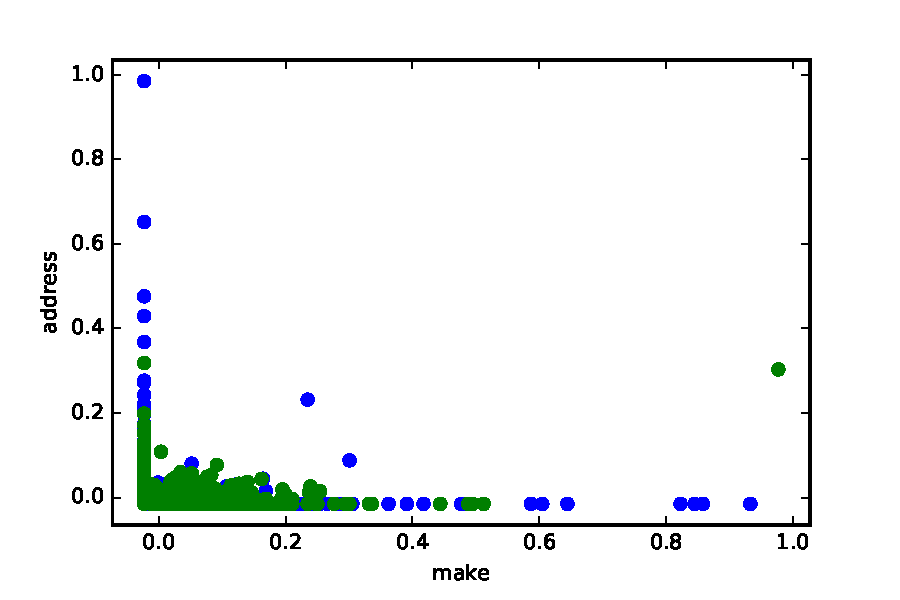
\includegraphics[width = 0.99\textwidth]{../../src/img/make_address.pdf}
  \end{minipage} \hfill
  \begin{minipage}{0.3\textwidth}
    b)\\
    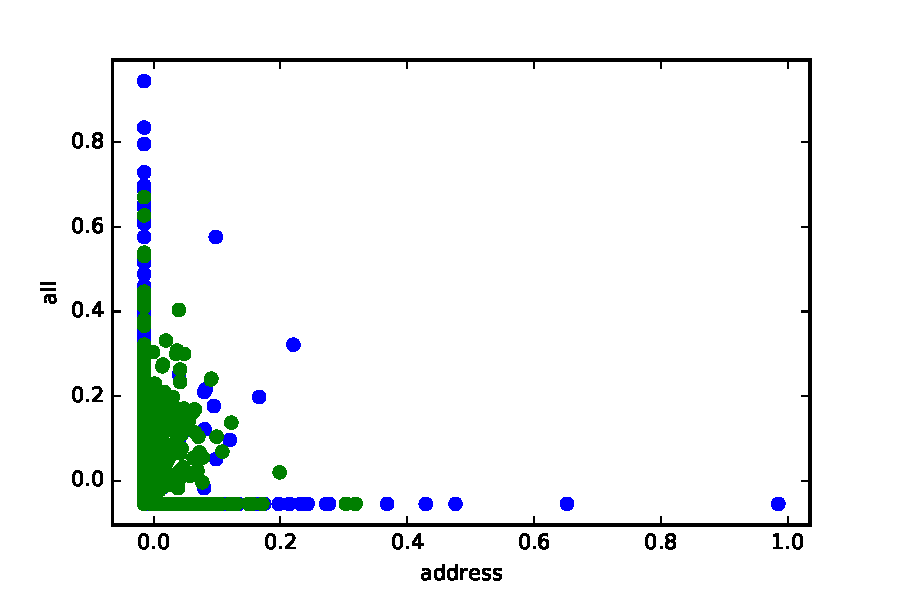
\includegraphics[width = 0.99\textwidth]{../../src/img/address_all.pdf}
  \end{minipage} \hfill
  \begin{minipage}{0.3\textwidth}
    c)\\
    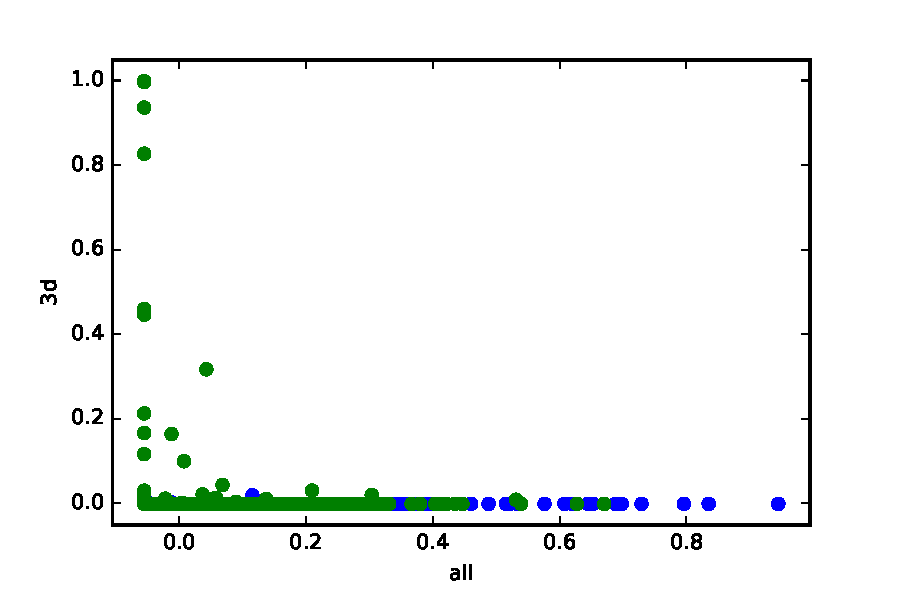
\includegraphics[width = 0.99\textwidth]{../../src/img/all_3d.pdf}
  \end{minipage} \vfill
  \begin{minipage}{0.3\textwidth}
    d)\\
    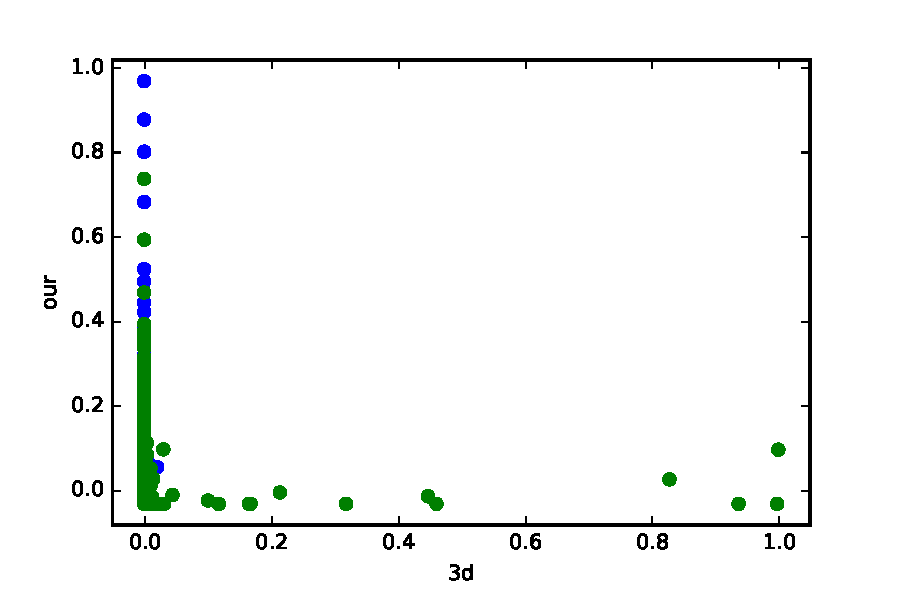
\includegraphics[width = 0.99\textwidth]{../../src/img/3d_our.pdf}
  \end{minipage} \hfill
  \begin{minipage}{0.3\textwidth}
    e)\\
    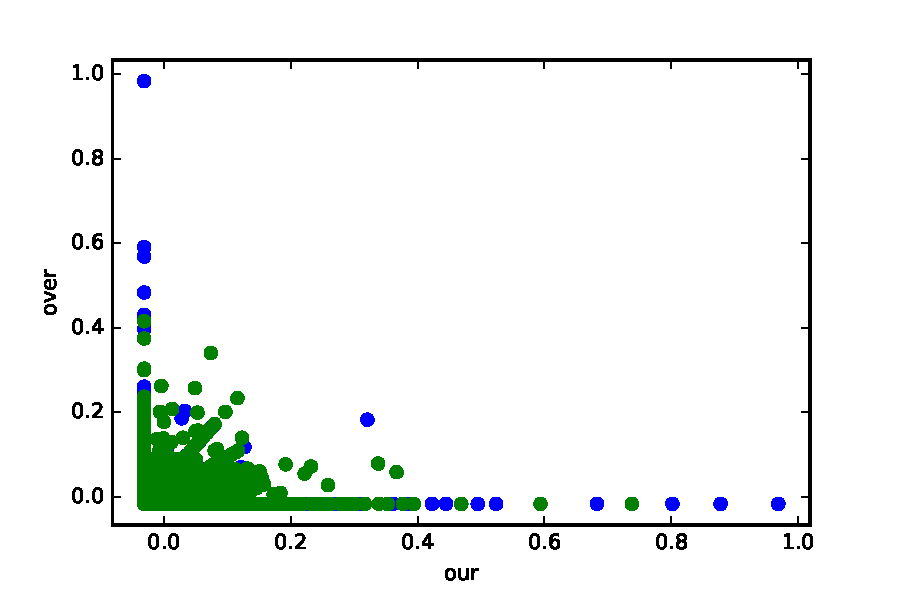
\includegraphics[width = 0.99\textwidth]{../../src/img/our_over.pdf}
  \end{minipage} \hfill
  \begin{minipage}{0.3\textwidth}
    f)\\
    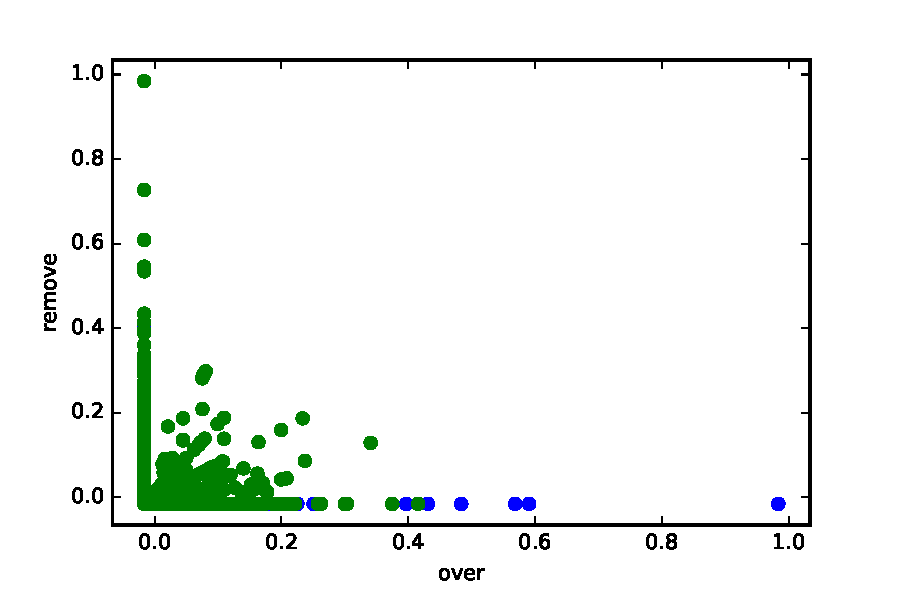
\includegraphics[width = 0.99\textwidth]{../../src/img/over_remove.pdf}
  \end{minipage} \vfill
  \caption{\label{fig:modelcheck} Green is spam and blue is not.}
\end{figure}

From this we can see that the spam and nonspam is hard to distinguish
just using one feature. But it is possible to see some patter as the
spam is slighly less spread than nonspam.
\newpage
To figure out what features to use with LR we do forward selection
with a 10-fold cross-validation. Intially this would not run as the
initial loss with zero features had a lower error than any of the
features applied to it. Though to show that we forwar feature
selection on our dataset the inital loss was hardcoded
$loss\_record=[0.27]$.

\begin{figure}[h]
  \centering
  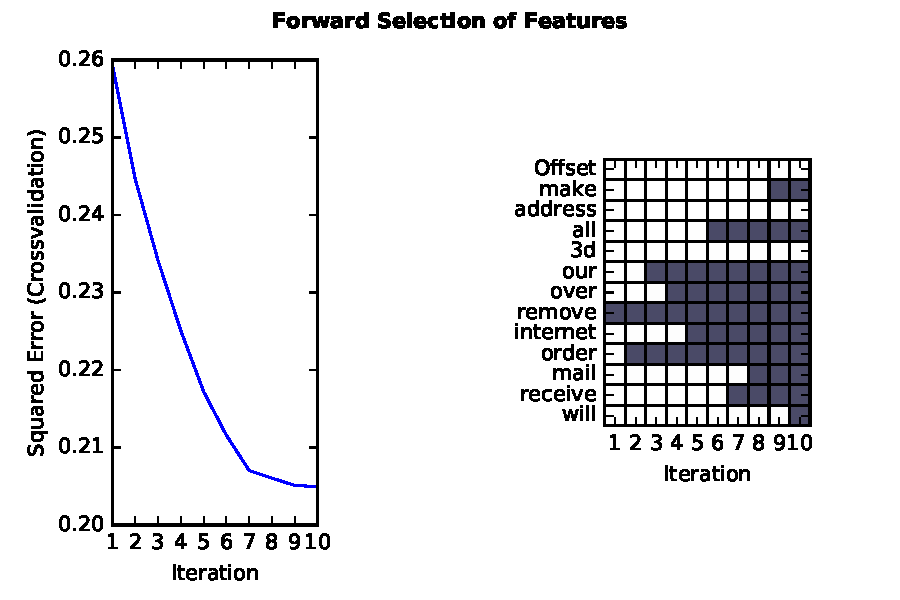
\includegraphics[width = 0.5\textwidth]{../../src/img/best_forward_selection.pdf}
  \caption{Forward selection form 12 features}
  \label{fig:gam}
\end{figure}

Above is the best feature selection that LRF could create with 12
features.  If we look at the error rates that are
computed:

\begin{figure}[h]
  \begin{minipage}{0.5\textwidth}
    \paragraph{Linear regression without feature selection:}
    \begin{itemize}
    \item Training error: 0.16731688100187755
    \item Test error:     0.1690774799900705
    \item $R^2$ train:     0.29925175624581624
    \item $R^2$ test:     0.2907848014802547
    \end{itemize}
  \end{minipage} \hfill
  \begin{minipage}{0.5\textwidth}
    \paragraph{Linear regression without feature selection:}
    \begin{itemize}
    \item Training error: 0.16731688100187755
    \item Test error:     0.1690774799900705
    \item $R^2$ train:     0.29925175624581624
    \item $R^2$ test:     0.2907848014802547
    \end{itemize}
  \end{minipage} \vfill
  \caption{Comparison of linear regression with and without feature selection}
\end{figure}

We can tell that without feature selection we get a smaller
error. Which leads us to believe that Linear Regression will not give
a great estimation of what is spam and what is not.

\subsection{Data predictions}
The fitted data has now created a model that can be used to fit the
email to spam or not.  The following vector are the coeficcients of
the trained model. These are the importance of each feature which in
turn helps us estimate if an email is spam or not.

\begin{table}[h]
  \centering
  \begin{tabular}{c|c|c|c|c|c|c|c|c|c|c}
    \hline Attribute & make & all & our & over & remove & internet & order
    & mail & receive & will \\ \hline Coefficient & 0.490 & 0.685 & 1.158
                                        & 1.631 & 2.510 & 2.079 & 1.237 & 0.958 & 0.660 & -0.279 \\ \hline
  \end{tabular}
  \caption{Training model coefficients}
\end{table}

Below, in figure~\ref{fig:residual-error} the residual error for the different fearures can
be seen. From these we can conclued that something causes something
but they do not show any distinct patterns.

\begin{figure}[h]
  \centering
  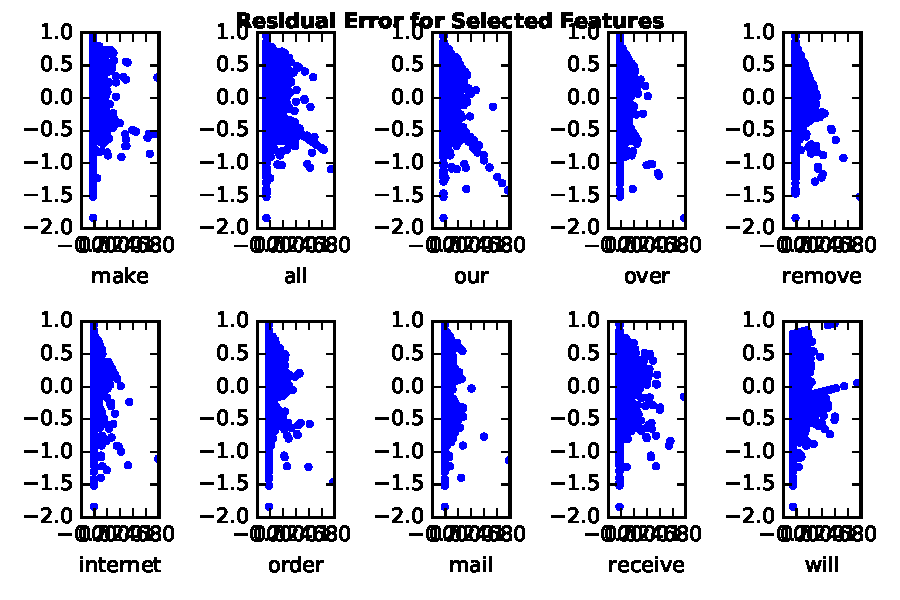
\includegraphics[width = 0.5\textwidth]{../../src/img/residual_error.pdf}
  \caption{\label{fig:residual-error} Residual error}
\end{figure}


\clearpage
\section{Classification}

\subsection{Problem}
We have chosen to solve the classification using Decision Trees,
K-Nearest Neighbors and Naive Bayes, all using K-Fold cross
validation.


%%%%%%%%%%%%%%%%%%%% Bibliography %%%%%%%%%%%%%%%%%%%%
\clearpage
\begin{thebibliography}{10}
\bibitem{datadescription} \url{http://archive.ics.uci.edu/ml/datasets/Abalone}
\bibitem{gam} \url{https://en.wikipedia.org/wiki/Generalized_additive_model}
\bibitem{Waugh.thesis} S.~Waugh,''Extending and Benchmark
  Cascade-Correlation,'' Thesis, 1997.
\bibitem{Mayukh} H.~Mayukh, ``Age of Abalones using Physical
  Characteristics: A Classification Problem,'' ECE 539 Fall 2010
  Project Report, Department of Electrical and Computer Engineering
  University of Wisconsin-Madison, 2010.
\end{thebibliography}
\end{document}
